\section{Riemann Sums} \label{S:4.2.Riemann}

\begin{goals}
\item How can we use a Riemann sum to estimate the area between a given curve and the horizontal axis over a particular interval?
\item What are the differences among left, right, middle, and random Riemann sums?
\item What is sigma notation and how does this enable us to write Riemann sums in an abbreviated form?
\end{goals}

%----------------------------------
% SUBSECTION INTRODUCTION
%----------------------------------
\subsection*{Introduction}

\begin{marginfigure}[3in] % MARGIN FIGURE
\margingraphics{figs/4/4-2_Intro.pdf}
\caption{A velocity function that is sometimes negative.} \label{fig:4.2_Intro}
\end{marginfigure}

In Section~\ref{S:4.1.VelocityDistance}, we learned that if we have a moving object with velocity function $v$, whenever $v(t)$ is positive, the area between $y = v(t)$ and the $t$-axis over a given time interval tells us the distance traveled by the object over that time period; in addition, if $v(t)$ is sometimes negative and we view the area of any region below the $t$-axis as having an associated negative sign, then the sum of these signed areas over a given interval tells us the moving object's change in position over the time interval.

For instance, for the velocity function given in Figure~\ref{fig:4.2_Intro}, if the areas of shaded regions are $A_1$, $A_2$, and $A_3$ as labeled, then the total distance $D$ traveled by the moving object on $[a,b]$ is 
\[D = A_1 + A_2 + A_3,\]
while the total change in the object's position on $[a,b]$ is 
\[s(b) - s(a) = A_1 - A_2 + A_3.\]
Because the motion is in the negative direction on the interval where $v(t) < 0$, we subtract $A_2$ when determining the object's total change in position.

Of course, finding $D$ and $s(b)-s(a)$ for the situation given in Figure~\ref{fig:4.2_Intro} presumes that we can actually find the areas represented by $A_1$, $A_2$, and $A_3$.  In most of our work in Section~\ref{S:4.1.VelocityDistance}, such as in Activities~\ref{A:4.1.2} and~\ref{A:4.1.3}, we worked with velocity functions that were either constant or linear, so that by finding the areas of rectangles and triangles, we could find the area bounded by the velocity function and the horizontal axis exactly.  But when the curve that bounds a region is not one for which we have a known formula for area, we are unable to find this area exactly.  Indeed, this is one of our biggest goals in Chapter~\ref{CH:4}: to learn how to find the exact area bounded between a curve and the horizontal axis for as many different types of functions as possible.  

To begin, we expand on the ideas in Activity~\ref{A:4.1.1}, where we encountered a nonlinear velocity function and approximated the area under the curve using four and eight rectangles, respectively.  In the following preview activity, we focus on three different options for deciding how to find the heights of the rectangles we will use.

\begin{marginfigure}[2cm] % MARGIN FIGURE
\captionsetup[subfigure]{labelformat=empty}
\begin{center}
\subfloat{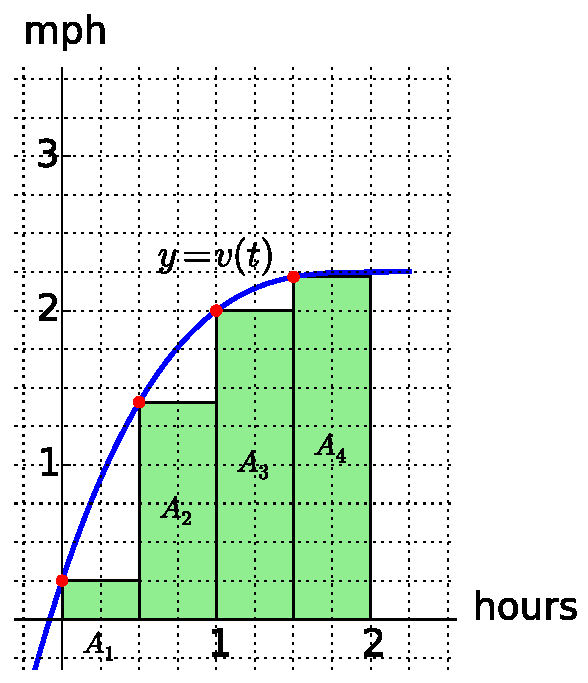
\includegraphics[scale=.5]{figs/4/preview_4-2a.pdf}}

\subfloat{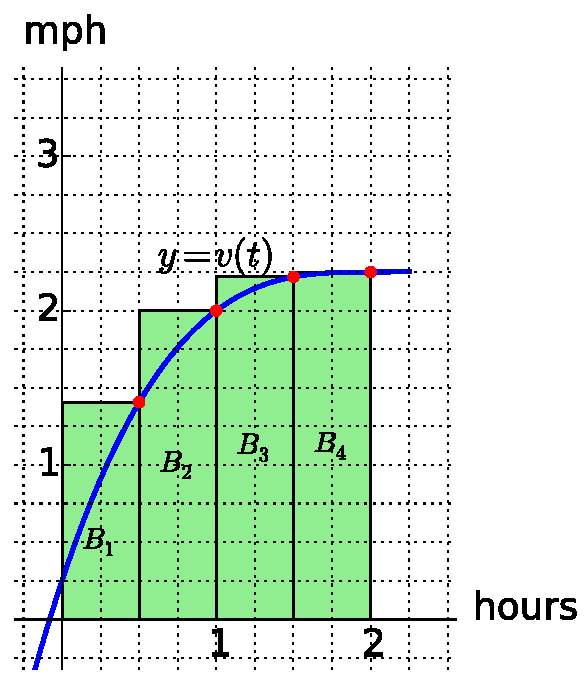
\includegraphics[scale=.5]{figs/4/preview_4-2b.pdf}}

\subfloat{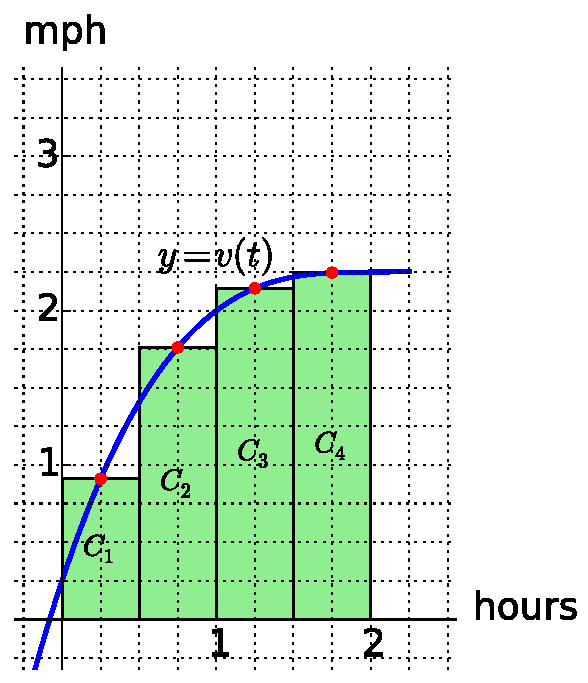
\includegraphics[scale=.5]{figs/4/preview_4-2c.pdf}}
\caption{Estimating the area under $y = v(t)$.} \label{fig:4.2.PA1}
\end{center}
\end{marginfigure}

%\begin{marginfigure} % MARGIN FIGURE
%\captionsetup[subfigure]{labelformat=empty}
%\subfloat{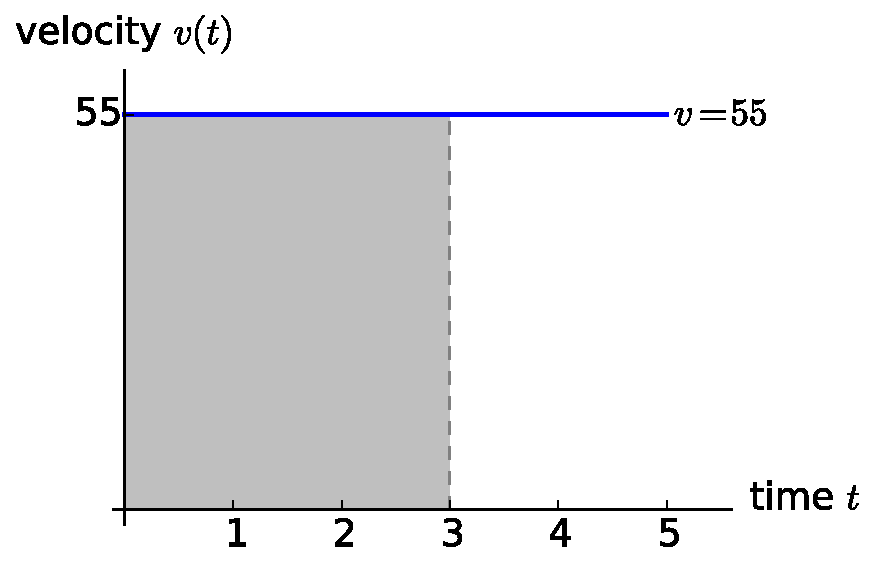
\includegraphics[width=\marginparwidth]{figs/0/position_t3.pdf}}
%
%\subfloat{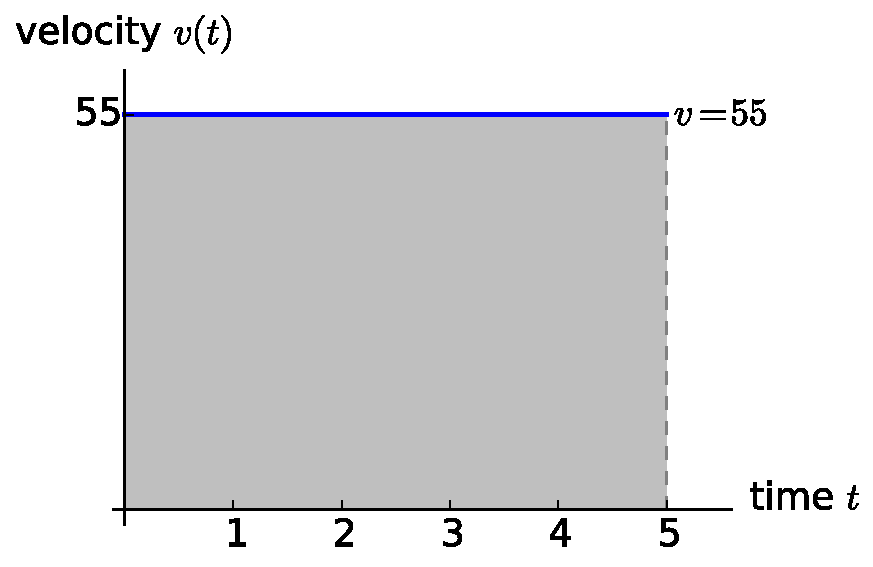
\includegraphics[width=\marginparwidth]{figs/0/position_t5.pdf}}
%\caption{Position at $t=3$ and $t=5$ represented by the area of a rectangle.}
%\label{fig:0-position_t5}
%\end{marginfigure}

\begin{pa} \label{PA:4.2}
A person walking along a straight path has her velocity in miles per hour at time $t$ given by the function $v(t) = 0.25t^3-1.5t^2+3t+0.25$, for times in the interval $0 \le t \le 2$.  The graph of this function is also given in each of the three diagrams. Note that in each diagram, we use four rectangles to estimate the area under $y = v(t)$ on the interval $[0,2]$, but the method by which the four rectangles' respective heights are decided varies among the three individual graphs.
\ba
\item How are the heights of rectangles in the left-most diagram being chosen?  Explain, and hence determine the value of 
\[ S = A_1 + A_2 + A_3 + A_4 \]
by evaluating the function $y = v(t)$ at appropriately chosen values and observing the width of each rectangle.  Note, for example, that 
\[ A_3 = v(1) \cdot \frac{1}{2} = 2 \cdot \frac{1}{2} = 1. \]

\item Explain how the heights of rectangles are being chosen in the middle diagram and find the value of
\[ T = B_1 + B_2 + B_3 + B_4. \]

\item Likewise, determine the pattern of how heights of rectangles are chosen in the right-most diagram and determine
\[ U = C_1 + C_2 + C_3 + C_4. \]
	
\item Of the estimates $S$, $T$, and $U$, which do you think is the best approximation of $D$, the total distance the person traveled on $[0,2]$?  Why?
\ea
\end{pa} 
\afterpa % PREVIEW ACTIVITY

%\begin{marginfigure} % MARGIN FIGURE
%\margingraphics{figs/4/apex_5-3_Area1.pdf}
%\caption{A graph of $f(x) = 4x-x^2$. What is the area of the shaded region?} \label{fig:apex_5-3_Area1}
%\end{marginfigure}
%
%\begin{marginfigure} % MARGIN FIGURE
%\margingraphics{figs/4/apex_5-3_Area1Approx.pdf}
%\caption{Approximating the area under $y=4x-x^2$ on $[0,4]$ using rectangles. The heights of the rectangles are determined using different methods.} \label{fig:apex_5-3_Area1Approx}
%\end{marginfigure}
%
%%A fundamental calculus technique is to first answer a given problem with an approximation, then refine that approximation to make it better, then use limits in the refining process to find the exact answer. That is exactly what we will do here.
%%
%%Consider the region given in Figure \ref{fig:apex_5-3_Area1}, which is the area under $y=4x-x^2$ on $[0,4]$. What is the signed area of this region? %-- i.e., what is $\int_0^4(4x-x^2)\ dx$?
%%
%%We start by approximating. We can surround the region with a rectangle with height and width of 4 and find the area is approximately 16 square units. This is obviously an \textit{over approximation}; we are including area in the rectangle that is not under the parabola. % do we need a picture?
%%
%%We have an approximation of the area, using one rectangle. How can we refine our approximation to make it better? The key to this section is this answer: \textit{use more rectangles.}
%%
%%Let's use 4 rectangles of equal width of 1. This \textit{partitions} the interval $[0,4]$ into 4 \textit{subintervals}, $[0,1]$, $[1,2]$, $[2,3]$ and $[3,4]$. On each subinterval we will draw a rectangle.
%
%There are three common ways to determine the height of these rectangles: the \textbf{Left Hand Rule}, the \textbf{Right Hand Rule}, and the \textbf{Midpoint Rule}. The \textbf{Left Hand Rule} says to evaluate the function at the left--hand endpoint of the subinterval and make the rectangle that height. In Figure \ref{fig:apex_5-3_Area1Approx}, the rectangle drawn on the interval $[2,3]$ has height determined by the Left Hand Rule; it has a height of $f(2)$. (The rectangle is labeled ``LHR.'')\index{Left Hand Rule}\index{Right Hand Rule}\index{Midpoint Rule}
%
%%\mfigure{.5}{Approximating the area under $y=4x-x^2$ on $[0,4]$ using rectangles. The heights of the rectangles are determined using different rules.}{fig:rie1b}{figures/figrie1b}
%
%The \textbf{Right Hand Rule} says the opposite: on each subinterval, evaluate the function at the right endpoint and make the rectangle that height. In the figure, the rectangle drawn on $[0,1]$ is drawn using $f(1)$ as its height; this rectangle is labeled ``RHR.''.
%
%The \textbf{Midpoint Rule} says that on each subinterval, evaluate the function at the midpoint and make the rectangle that height. The rectangle drawn on $[1,2]$ was made using the Midpoint Rule, with a height of $f(1.5)$. That rectangle is labeled ``MPR.''
%
%These are the three most common rules for determining the heights of approximating rectangles, but one is not forced to use one of these three methods. The rectangle on $[3,4]$ has a height of approximately $f(3.53)$, very close to the Midpoint Rule. It was chosen so that the area of the rectangle is \textit{exactly} the area of the region under $f$ on $[3,4]$. (Later you'll be able to figure how to do this, too.)
%
%The following example will approximate the value of the area under $y=4x-x^2$ on $[0,4]$ using these rules.

\begin{example} % EXAMPLE
Approximate the area of the region under $y=4x-x^2$ on the interval $[0,4]$ using $L_4$, $R_4$, and $M_4$. 

\solution We partition the interval $[0,4]$ into the four subintervals $[0,1]$, $[1,2]$, $[2,3]$, and $[3,4]$. In Figure~\ref{fig:apex_5-3_Area1}-(a) we see $4$ rectangles drawn on $f(x) = 4x-x^2$ using the $L_4$. Note how in the first subinterval, $[0,1]$, the rectangle has height $f(0)=0$. We add up the areas of each rectangle, which is width $\times$ height, for our $L_4$ approximation:
\begin{eqnarray*}
L_4 & = & 1 \cdot f(0) + 1 \cdot f(1)+ 1 \cdot f(2) + 1 \cdot f(3) \\
& = & 0+3+4+3 \\
& = & 10.
\end{eqnarray*}
	
Figure~\ref{fig:apex_5-3_Area1}-(b) shows $4$ rectangles drawn under $f$ using $R_4$; note how the rectangle on the subinterval $[3,4]$ has height $0$.  Our approximation gives the same answer as before, though calculated a different way:
\begin{eqnarray*}
R_4 & = & 1 \cdot f(1) + 1 \cdot f(2)+ 1 \cdot f(3) + 1 \cdot f(4) \\
& = & 3+4+3+0 \\
& = & 10.
\end{eqnarray*}

Figure~\ref{fig:apex_5-3_Area1}-(c) shows $4$ rectangles drawn under $f$ using $M_4$. Notice that the height of each of the rectangles is determined by the point in the middle of each subinterval, which are $0.5$, $1.5$, $2.5$, and $3.5$. So
\begin{eqnarray*}
M_4 & = & 1 \cdot f(0.5) + 1 \cdot f(1.5)+ 1 \cdot f(2.5) + 1 \cdot f(3.5) \\
& = & 1.75 + 3.75 + 3.75 + 1.75 \\
& = & 11.
\end{eqnarray*}
\end{example}

\begin{marginfigure} % MARGIN FIGURE
\begin{center}
%\captionsetup[subfigure]{labelformat=empty}
\subfloat[$L_n$]{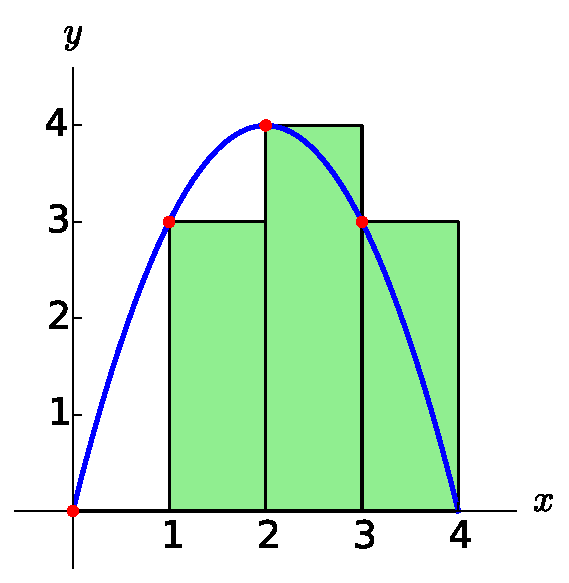
\includegraphics[scale=.5]{figs/4/apex_5-3_Area1Ln.pdf}}
%\caption{Approximating the area under $y=4x-x^2$ on $[0,4]$ using $L_n$} \label{fig:apex_5-3_Area1}

\subfloat[$R_n$]{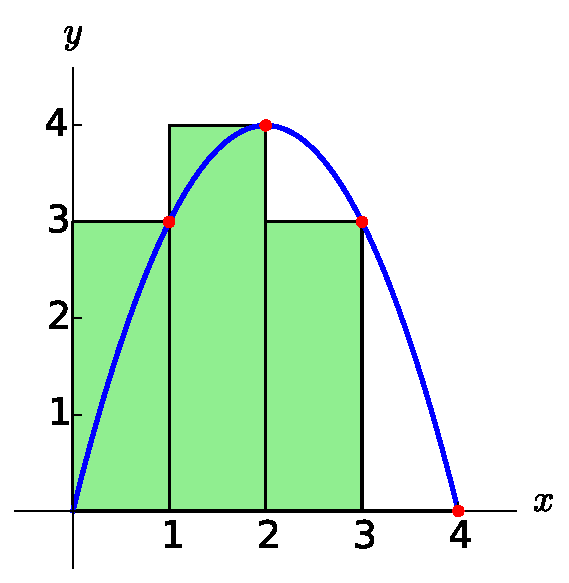
\includegraphics[scale=.5]{figs/4/apex_5-3_Area1Rn.pdf}}
%\caption{Approximating the area under $y=4x-x^2$ on $[0,4]$ using $R_n$} \label{fig:apex_5-3_Area1}

\subfloat[$M_n$]{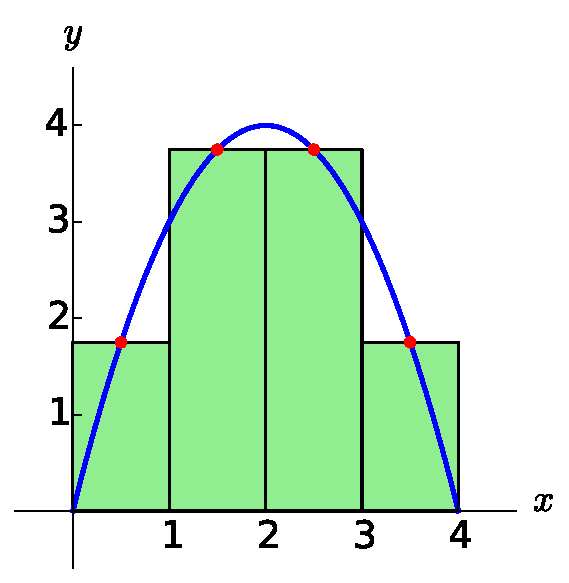
\includegraphics[scale=.5]{figs/4/apex_5-3_Area1Mn.pdf}}
\caption{Approximating the area under $y=4x-x^2$ on $[0,4]$ using $L_n$, $R_n$, and $M_n$} \label{fig:apex_5-3_Area1}
\end{center}
\end{marginfigure}

%-------------------------------------
% SUBSECTION SIGMA NOTATION
%-------------------------------------
\subsection*{Sigma Notation}

It is apparent from several different problems we have considered that sums of areas of rectangles is one of the main ways to approximate the area under a curve over a given interval.  Intuitively, we expect that using a larger number of thinner rectangles will provide a way to improve the estimates we are computing.  As such, we anticipate dealing with sums with a large number of terms.  To do so, we introduce the use of so-called \emph{sigma notation}\index{sigma notation}, named for the Greek letter $\Sigma$, which is the capital letter $S$ in the Greek alphabet.

For example, say we are interested in the sum
$$1 + 2 + 3 + \cdots + 100,$$
which is the sum of the first 100 natural numbers.  Sigma notation provides a shorthand notation that recognizes the general pattern in the terms of the sum.  It is equivalent to write
$$\sum_{k=1}^{100} k =  1 + 2 + 3 + \cdots + 100.$$
We read the symbol $\ds \sum_{k=1}^{100} k$ as ``the sum from $k$ equals 1 to 100 of $k$.''  The variable $k$ is usually called the index of summation, and the letter that is used for this variable is immaterial. 

Suppose we wish to add up a list of numbers $a_1$, $a_2$, $a_3$, \ldots, $a_9$. Instead of writing \[ a_1+a_2+a_3+a_4+a_5+a_6+a_7+a_8+a_9, \]
we use summation notation and write 
\[ \sum_{i=1}^9 a_i. \]
Again, the capital sigma represents the term ``sum.'' The index of summation in this example is $i$. By convention, the index takes on only the integer values between (and including) the lower and upper bounds. 

Each summand in sigma notation involves a function of the index; for example,
\begin{eqnarray*}
\sum_{k=1}^{10} (k^2 + 2k) & = & (1^2 + 2\cdot 1) + (2^2 + 2\cdot 2) + (3^2 + 2\cdot 3) \\
& & + \cdots + (10^2 + 2\cdot 10),
\end{eqnarray*}
and more generally,
$$\sum_{k=1}^n f(k) = f(1) + f(2) + \cdots + f(n).$$
Sigma notation allows us the flexibility to easily vary the function being used to track the pattern in the sum, as well as to adjust the number of terms in the sum simply by changing the value of $n$.  We test our understanding of this new notation in the following activity.

\begin{activity} \label{A:4.2.1}  For each sum written in sigma notation, write the sum long-hand and evaluate the sum to find its value.  For each sum written in expanded form, write the sum in sigma notation.
\ba
	\item $\ds \sum_{k=1}^{5} (k^2 + 2)$
	\item $\ds \sum_{i=3}^{6} (2i-1)$
	\item $\ds 3 + 7 + 11 + 15 +  \cdots + 27$
	\item $\ds 4 + 8 + 16 + 32 \cdots + 256$
	\item $\ds \sum_{i=1}^{6} \frac{1}{2^i}$
\ea
\end{activity}
\begin{smallhint}
\ba
	\item Observe that when $k = 1$, $k^2 + 2 = 1^2 + 2 = 3$.  This is the first term in the sum.
	\item Note that this sum starts at $i = 3$.
	\item Since the terms in the sum increase by 4, try a function $f(k)$ that somehow involves $4k$.
	\item What pattern do you observe in the terms of the sum?
	\item Write every term in the sum as a fraction with denominator $2^6 = 64$.
\ea
\end{smallhint}
\begin{bighint}
\ba
	\item Observe that when $k = 1$, $k^2 + 2 = 1^2 + 2 = 3$.  This is the first term in the sum.  The last term in the sum occurs when $k = 5$, which is $5^2 + 2 = 27$.
	\item Note that this sum starts at $i = 3$ and the first term is $(2\cdot 3 - 1) = 5$.
	\item Since the terms in the sum increase by 4, try a function $f(k)$ that somehow involves $4k$.  You have freedom to decide where your index $k$ starts; try $k = 1$.
	\item What pattern do you observe in the terms of the sum?
	\item Write every term in the sum as a fraction with denominator $2^6 = 64$.
\ea
\end{bighint}
\begin{activitySolution}
\ba
	\item 
	\begin{eqnarray*}
	 \sum_{k=1}^{5} (k^2 + 2) & = & (1^2 + 2) + (2^2 + 2) + (3^2 + 2) + (4^2 + 2) + (5^2 + 2) \\
	 					& = & 3 + 6 + 11 + 17 + 27 \\
						& = & 64
	\end{eqnarray*}
	\item 
	\begin{eqnarray*}
	 \sum_{i=3}^{6} (2i-1) & = & (2 \cdot 3 - 1) + (2 \cdot 4- 1) + (2 \cdot 5 - 1) + (2 \cdot 6 - 1) \\
	 				& = & 5 + 7 + 9 + 11 \\
					& = & 32
	\end{eqnarray*}
	\item Observe that each term in the sum
	$$\ds 3 + 7 + 11 + 15 +  \cdots + 27$$
	differs from the previous term by 4.  If we view $4$ as $4 = 4 \cdot 1 - 1$ and $7$ as $7 = 4 \cdot 2 - 1$, we see that the pattern may be represented through the function $f(k) = 4k-1$, so that
	$$\ds 3 + 7 + 11 + 15 +  \cdots + 27 = \sum_{k=1}^{7} 4k-1.$$
	We note that $k=7$ is the end value of the index since $4 \cdot 7  = 28$.
	\item The sum $\ds 4 + 8 + 16 + 32 + \cdots + 256$ is a sum of powers of $2$, which we can express in sigma notation as
	$$4 + 8 + 16 + 32 + \cdots + 256 = \sum{i=2}^{8} 2^i.$$
	\item
	\begin{eqnarray*}
	  \sum_{i=1}^{6} \frac{1}{2^i} & = & \frac{1}{2} + \frac{1}{2^2} + \cdots + \frac{1}{2^6} \\
	  					& = & \frac{32}{64} + \frac{16}{64} + \frac{8}{64} + \frac{4}{64} + \frac{2}{64} + \frac{1}{64} \\
						& = & \frac{63}{64}.
	\end{eqnarray*}
\ea
\end{activitySolution}
\aftera % ACTIVITY

It might seem odd to stress a new, concise way of writing summations only to write each term out as we add them up. It is. Therefore, we give some properties of summations that allow us to work with them without writing individual terms. 

\definition{Properties of Summations\index{summation!properties}}{
\begin{enumerate}
\item	$\ds \sum_{i=1}^n c = c\cdot n$, where $c$ is a constant.
\item	$\ds \sum_{i=m}^n (a_i\pm b_i) = \sum_{i=m}^n a_i \pm \sum_{i=m}^n b_i$
\end{enumerate}
\begin{multicols}{2}
\begin{enumerate}[resume]

\item	$\ds \sum_{i=1}^n c\cdot a_i = c\cdot\sum_{i=1}^n a_i$
\item	$\ds \sum_{i=m}^j a_i + \sum_{i=j+1}^n  a_i = \sum_{i=m}^n a_i$
\item	$\ds \sum_{i=1}^n i = \frac{n(n+1)}2$
\item	$\ds \sum_{i=1}^n i^2 = \frac{n(n+1)(2n+1)}6$
\item	$\ds \sum_{i=1}^n i^3 = \left(\frac{n(n+1)}2\right)^2$
\end{enumerate}
\end{multicols}
$\left.\right.$
}\pagebreak

\begin{example} % EXAMPLE
Evaluate $\ds  \sum_{i=1}^6 (2i-1)$. 

\solution 
\begin{align*}
\sum_{i=1}^6 (2i-1) & = \sum_{i=1}^6 2i - \sum_{i=1}^6 1 \\
& = 2\sum_{i=1}^6 i - \sum_{i=1}^6 1 \\
& = 2 \left( \frac{6(6+1)}{2} \right) - 6 \\
& = 42-6 \\
& = 36
\end{align*}
We obtained the same answer without writing out all six terms. When dealing with small sizes of $n$, it may be faster to write the terms out by hand. However, the Properties of Summations are incredibly important when dealing with large sums as we'll soon see.
\end{example}

%%----------------------------------
%% SUBSECTION RIEMANN SUMS
%%----------------------------------
%\subsection*{Riemann Sums}
%
%Consider again the area under $y=4x-x^2$ on $[0,4]$. We will approximate this area using 16 equally spaced subintervals and the Right Hand Rule in Example \ref{ex_rie7}. Before doing so, it will pay  to do some careful preparation.\index{Riemann Sum}
%
%%\mfigure{.5}{Dividing $[0,4]$ into 16 equally spaced subintervals.}{fig:rie5}{figures/figrie5}
%
%Figure \ref{fig:rie5} shows a number line of $[0,4]$ divided into 16 equally spaced subintervals. We denote $0$ as $x_1$; we have marked the values of $x_5$, $x_9$, $x_{13}$ and $x_{17}$. We could mark them all, but the figure would get crowded. While it is easy to figure that $x_{10} = 2.25$, in general, we want a method of determining the value of $x_i$ without consulting the figure. Consider:
%	%\begin{center}\myincludegraphics{figures/figrie5a}\end{center}
%	%$$x_i = x_1 + (i-1)\Delta x. \text{TIKZ}$$
%So $x_{10} = x_1 + 9(4/16) = 2.25.$
%
%If we had partitioned $[0,4]$ into 100 equally spaced subintervals, each subinterval would have length $\Delta x=4/100 = 0.04$. We could compute $x_{32}$ as $$x_{32} = x_1 + 31(4/100) = 1.24.$$ (That was far faster than creating a sketch first.)
%
%Given any subdivision of $[0,4]$, the first subinterval is $[x_1,x_2]$; the second is $[x_2,x_3]$; the $i^\text{ th}$ subinterval is $[x_i,x_{i+1}]$. 
%
%When using the Left Hand Rule, the height of the $i^\text{ th}$ rectangle will be $f(x_i)$. 
%
%When using the Right Hand Rule, the height of the $i^\text{ th}$ rectangle will be $f(x_{i+1})$. 
%
%When using the Midpoint Rule, the height of the $i^\text{ th}$ rectangle will be $\ds f\left(\frac{x_i+x_{i+1}}2\right)$. 
%
%Thus approximating the area under $y=4x-x^2$ on $[0,4]$ with 16 equally spaced subintervals can be expressed as follows:\vskip 5pt
%
%\noindent \textbf{Left Hand Rule:} $L_{16} = \ds \sum_{i=1}^{16} f(x_i)\Delta x$ \vskip 5pt
%
%\noindent \textbf{Right Hand Rule:} $R_{16} = \ds \sum_{i=1}^{16} f(x_{i+1})\Delta x$\vskip 5pt
%
%\noindent \textbf{Midpoint Rule:} $M_{16}\ds \sum_{i=1}^{16} f\left(\frac{x_i+x_{i+1}}2\right)\Delta x$
%\index{Left Hand Rule}\index{Right Hand Rule}\index{Midpoint Rule}

%\begin{marginfigure}[8cm] % MARGIN FIGURE
\margingraphics{figs/4/apex_5-3_Area1Rn16.pdf}
\caption{Approximating the area under $y~=~4x-x^2$ on $[0,4]$ using $R_n$ with $n=16$.} \label{fig:apex_5-3_Area1Rn16}
\end{marginfigure}

\begin{example} % EXAMPLE
Approximate the area under $y=4x-x^2$ on $[0,4]$ using $R_n$ and summation formulas with $16$ and $1000$ equally spaced intervals.

\solution Using $16$ rectangles, we can approximate the area as 
\[ \sum_{i=1}^{16} f(x_i) \Delta x \]
where $\Delta x = 4/16 = 1/4$ and $x_i = 0 + i \Delta x = i \Delta x$. Using the properties of summations, we have
\begin{eqnarray}
\mbox{Area} & \approx & R_{16}  = \sum_{i=1}^{16} f(x_i) \Delta x \notag \\
&=& \sum_{i=1}^{16} f( i\Delta x ) \Delta x \notag \\
&=& \sum_{i=1}^{16} \left( 4i \Delta x - (i \Delta x)^2 \right) \Delta x \notag \\
&=& \sum_{i=1}^{16} \left( 4i \Delta x^2 - i^2 \Delta x^3 \right) \notag \\		
&=& \left( 4\Delta x^2 \right) \sum_{i=1}^{16} i - \left( \Delta x^3 \right) \sum_{i=1}^{16} i^2 \label{eq:rie7} \\ %\label{eq:rie7}
&=& (4\Delta x^2)\frac{16\cdot 17}{2} - \left( \Delta x^3 \right) \frac{16(17)(33)}6 \notag \\
&=&	4 \cdot \left( \frac{1}{4} \right)^2 \cdot \frac{16\cdot 17}{2} - \left( \frac{1}{4} \right)^3 \cdot \frac{16(17)(33)}{6} \notag \\
&=&	2 \cdot 17 - \frac{17 \cdot 11}{8} \notag \\
&=& \frac{85}{8} = 10.625 \notag
\end{eqnarray}
We were able to sum up the areas of $16$ rectangles with very little computation. Notice  Equation \eqref{eq:rie7}; by changing the $16$'s to $1,000$'s (and appropriately changing the value of $\Delta x$ to $4/1000$), we can use that equation to sum up $1000$ rectangles!
\begin{align*}
\mbox{Area} & \approx R_{1000} = \sum_{i=1}^{1000} f(x_i) \Delta x \\
&= \left( 4 \Delta x^2 \right) \sum_{i=1}^{1000} i - \left(\Delta x^3 \right) \sum_{i=1}^{1000} i^2 \\
&= \left( 4 \Delta x^2 \right) \frac{1000 \cdot 1001}{2} - \left( \Delta x^3 \right) \frac{1000(1001)(2001)}6 \\
&= 4 \cdot (0.004)^2 \cdot 500500 - (0.004)^3\cdot 333,833,500\\
&= 10.666656
\end{align*}

Using this many rectangles, it's likely that we have a good approximation of the area under $y=4x-x^2$ on $[0,4]$. That is, the area is approximately $10.666656$.
\end{example}

%\begin{activity} \label{A:4.2.2}  Suppose that an object moving along a straight line path has its velocity in feet per second at time $t$ in seconds given by $\ds v(t) = \frac{2}{9}(t-3)^2 + 2$.
\ba
\item Carefully sketch the region whose exact area will tell you the value of the distance the object traveled on the time interval $2 \le t \le 5$.
	
\item Estimate the distance traveled on $[2,5]$ by computing $L_4$, $R_4$, and $M_4$.

\item Does averaging $L_4$ and $R_4$ result in the same value as $M_4$?  If not, what do you think the average of $L_4$ and $R_4$ measures?

\item For this question, think about an arbitrary function $f$, rather than the particular function $v$ given above.  If $f$ is positive and increasing on $[a,b]$, will $L_n$ over-estimate or under-estimate the exact area under $f$ on $[a,b]$?  Will $R_n$ over- or under-estimate the exact area under $f$ on $[a,b]$? Explain.
\ea
\end{activity}

\begin{smallhint}
\ba
	\item Note that $y = v(t)$ is a parabola with vertex $(3,2)$.
	\item Recall the formulas for $L_n$, $R_n$, and $M_n$.
	\item Think about what the average of $L_1$ and $R_1$ measures.
	\item Consider carefully the role of endpoints in generating $L_n$ and $R_n$.
\ea
\end{smallhint}
\begin{bighint}
\ba
	\item Note that $y = v(t)$ is a parabola with vertex $(3,2)$.
	\item Recall the formulas for $L_n$, $R_n$, and $M_n$.
	\item Think about what the average of $L_1$ and $R_1$ measures.
	\item Consider carefully the role of endpoints in generating $L_n$ and $R_n$ and what you know about the behavior of an always increasing function.
\ea
\end{bighint}
\begin{activitySolution}
\ba
	\item The region whose exact area tells us the value of the distance the object traveled on the time interval $2 \le t \le 5$ is shown below.
	\begin{center}
		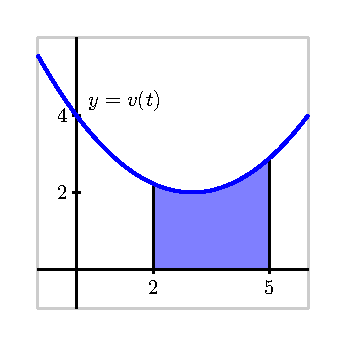
\includegraphics{figures/4_2_Act2Soln.eps}
	\end{center}
	\item $L_4 = \frac{311}{48} \approx 6.47917$, 
	        $R_4 = \frac{335}{48} \approx 6.97917$, and 
	        $M_4 = \frac{637}{96} \approx 6.63542$.
	\item The average of $L_4$ and $R_4$ is
	$$\frac{L_4 + M_4}{2} = \frac{311+335}{96} = \frac{646}{96} \ne \frac{637}{96} = M_4.$$
	This average actually measures what would result from using four trapezoids, rather than rectangles, to estimate the area on each subinterval.  One reason this is so is because the area of a trapezoid is the average of the bases times the width, and the ``bases'' are given by the function values at the left and right endpoints.
	\item If $f$ is positive and increasing on $[a,b]$, $L_n$ will under-estimate the exact area under $f$ on $[a,b]$.  Because $f$ is increasing, its value at the left endpoint of any subinterval will be lower than every other function value in the interval, and thus the rectangle with that height lies exclusively below the curve.  In a similar way, $R_n$ over-estimates the exact area under $f$ on $[a,b]$.
\ea
\end{activitySolution}
\aftera % ACTIVITY
%
%Before the above example, we stated what the summations for the Left Hand, Right Hand and Midpoint Rules looked like. Each had the same basic structure; the only difference was at what values to evaluate $f$. All three are examples of an even more general construction, named after mathematician Georg Friedrich Bernhard Riemann.
%
%\definition{Riemann Sum}
%{Let $f$ be defined on the closed interval $[a,b]$ and let $\Delta x$ be a partition of $[a,b]$, with \index{Riemann Sum}
%	$$a=x_1 < x_2 < \ldots < x_n < x_{n+1}=b.$$
%Let $\Delta x_i$ denote the length of the $i^\text{ th}$ subinterval $[x_i,x_{i+1}]$ and let $c_i$ denote any value in the $i^\text{ th}$ subinterval.
%
%The sum $$\sum_{i=1}^n f(c_i)\Delta x_i$$  is a \textbf{Riemann sum} of $f$ on $[a,b]$.}
%
%In this general form, the subintervals do not have be of equal length, and one can choose a point $c_i$ inside each subinterval any way they choose (and not just the left endpoint, or the midpoint, etc.) Figure \ref{fig:riedef} shows the approximating rectangles of a Riemann sum of the area under $y=4x-x^2$ on $[0,4]$. (This particular approximation is of little use; clearly the width and heights of the rectangles were not chosen ``well.'')
%
%%\mfigure{.55}{An example of a general Riemann sum to approximate the area under $y=4x-x^2$ on $[0,4]$.}{fig:riedef}{figures/figriedef}
%
%``Usually'' Riemann sums are calculated using one of the three methods we have introduced. The uniformity of construction  makes computations easier. Before working another example, let's summarize some of what we have learned in a convenient way.
%
%\concept{Riemann Sum Concepts}{Let $A$ be the area under the curve $f(x)$. Consider the approximation $A \approx \sum_{i=1}^n f(c_i)\Delta x_i.$ 
%
%\begin{enumerate}
%\item	When the $n$ subintervals have equal length, $\ds \Delta x_i = \Delta x = \frac{b-a}n.$
%\item		The $i^\text{ th}$ term of the partition is $x_i = a + (i-1)\Delta x$. (This makes $x_{n+1} = b$.)
%\item		The Left Hand Rule summation is: $\ds \sum_{i=1}^n f(x_i)\Delta x$.
%\item		The Right Hand Rule summation is: $\ds \sum_{i=1}^n f(x_{i+1})\Delta x$.
%\item		The Midpoint Rule summation is: $\ds \sum_{i=1}^n f\left(\frac{x_i+x_{x+1}}{2}\right)\Delta x$.
%\end{enumerate}
%%\textit{\small (continued $\ldots$)}
%}
%
\pagebreak
\begin{marginfigure}[7cm] % MARGIN FIGURE
\margingraphics{figs/4/apex_5-3_Area2M.pdf}
\caption{Approximating net signed area of $f(x)=5x+2$ using the Midpoint Rule and $10$ evenly spaced subintervals.} \label{fig:apex_5-3_Area2M}
\end{marginfigure}

\begin{example}\label{eg:NetAreaM10} % EXAMPLE
Approximate the net area between $f(x)= 5x+2$ and the $x$-axis on $[-2,3]$ using the Midpoint Rule and 10 equally spaced intervals.

\solution Beginning with $\Delta x$ and $x_i$, we have
\[ \Delta x = \frac{3 - (-2)}{10} = \frac{1}{2} \quad \text{and} \quad x_i = -2 + \frac{1}{2} \cdot i = \frac{i}{2} - 2.\]
As we are using the Midpoint Rule, we will also need $x_{i-1}$ and $\ds \frac{x_{i-1}+x_i}{2}$. Since $\ds x_i = \frac{i}{2} - 2$,  $\ds x_{i-1} =\frac{i-1}{2} - 2 = \frac{i}{2} - \frac{5}{2}$.
Then 
\[ \frac{x_{i-1}+x_i}{2} = \frac{\ds\frac{i}{2} - \frac{5}{2} +\frac{i}{2} - 2}{2} = \frac{\ds i-\frac{9}{2}}{2} = \frac{i}{2} - \frac{9}{4}.\]
We now construct the Riemann sum and compute its value using summation formulas.
\begin{align*}
\mbox{Area} & \approx M_{10} = \sum_{i=1}^{10} f\left( \frac{x_{i-1}+x_i}{2} \right) \Delta x \\
&=	\sum_{i=1}^{10} f \left( \frac{i}{2} - \frac{9}{4} \right) \Delta x \\
&=	\sum_{i=1}^{10} \left( 5 \left( \frac{i}{2} - \frac{9}{4} \right) + 2 \right) \Delta x \\
&=	\Delta x\sum_{i=1}^{10}\left[\left(\frac{5}{2}\right)i - \frac{37}{4}\right]\\
&=	\Delta x\left(\frac{5}2\sum_{i=1}^{10} (i) - \sum_{i=1}^{10}\left(\frac{37}{4}\right)\right) \\
&= \frac12\left(\frac52\cdot\frac{10(11)}{2} - 10\cdot\frac{37}4\right)  \\
&= \frac{45}2 = 22.5.
\end{align*}
\end{example}

%
%Notice in the previous example that while we used 10 equally spaced intervals, the number ``10'' didn't play a big role in the calculations until the very end. Mathematicians love to abstract ideas; let's approximate another region using $n$ subintervals, where we do not specify a value of $n$ until the very end.
\pagebreak
\begin{example} % EXAMPLE
Approximate the net area of $f(x)=4x-x^2$ on $[0,4]$ again using $R_n$ with $n$ rectangles. 

\solution We have 
\[ \Delta x = \frac{4-0}{n} = \frac{4}{n} \quad \mbox{and} \quad x_i = 0 + i \Delta x = \frac{4}{n}i,\]
and we approximate the area as
\begin{align*}
A &\approx \sum_{i=1}^n f(x_i) \Delta x \\
&= \sum_{i=1}^n f \left( \frac{4}{n}i \right) \Delta x \\
&= \Delta x \sum_{i=1}^n \left[ 4 \cdot \frac{4}{n}i - \left( \frac{4}{n}i \right)^2 \right]  \\
&= \Delta x \left[ \sum_{i=1}^n \left(\frac{16}{n}\right)i - \sum_{i=1}^n \left(\frac{16}{n^2}\right)i^2 \right] \\
&= \frac{16\Delta x}{n} \left[ \sum_{i=1}^n i - \frac{1}{n} \sum_{i=1}^n i^2 \right]  \\
&= \frac{64}{n^2} \left[ \frac{n(n+1)}{2} - \frac{1}{n} \cdot \frac{n(n+1)(2n+1)}{6} \right] \\
&= \frac{32(n+1)}{n} - \frac{32(n+1)(2n+1)}{3n^2} \\
&= \frac{32}{3}\left(1-\frac{1}{n^2}\right)
\end{align*}
\end{example}

%The result is an amazing, easy to use formula. To approximate the area with 10 equally spaced subintervals and the Right Hand Rule, set $n=10$ and compute $$A \approx \frac{32}{3}\left(1-\frac{1}{10^2}\right) = 10.56.$$
%Recall how earlier we approximated the area with 4 subintervals; with $n=4$, the formula gives 10, our answer as before.
%
%It is now easy to approximate the area with 1,000,000 subintervals!  Hand-held calculators will round off the answer a bit prematurely giving an answer of $10.66666667$. (The actual answer is $10.666666666656$.)
%
%We now take an important leap. Up to this point, our mathematics has been limited to geometry and algebra (finding areas and manipulating expressions). Now we apply \textit{calculus}. For any \textit{finite} $n$, we know that the area, $A$, between $f(x)=4x-x^2$ and the $x$ axis is $$A \approx \frac{32}{3}\left(1-\frac{1}{n^2}\right).$$ Both common sense and high--level mathematics tell us that as $n$ gets large, the approximation gets better. In fact, if we take the \textit{limit} as $n\rightarrow \infty$, we get the \textit{exact area}. That is, 
%\begin{align*}
%A &= \lim_{n\rightarrow \infty} \frac{32}{3}\left(1-\frac{1}{n^2}\right) \\
%									&= \frac{32}{3}\left(1-0\right)\\
%									&= \frac{32}{3} = 10.\overline{6}
%\end{align*}
%
%
%\begin{activity} \label{A:4.2.3}  Suppose that an object moving along a straight line path has its velocity $v$ (in feet per second) at time $t$ (in seconds) given by 
\[ v(t) = \frac{1}{2}t^2 - 3t + \frac{7}{2}. \]
\ba
\item Compute $M_5$, the middle Riemann sum, for $v$ on the time interval $[1,5]$.  Be sure to clearly identify the value of $\triangle t$ as well as the locations of $t_0$, $t_1$, $\cdots$, $t_5$.  In addition, provide a careful sketch of the function and the corresponding rectangles that are being used in the sum.

\item Building on your work in (a), estimate the total change in position of the object on the interval $[1,5]$.

\item Building on your work in (a) and (b), estimate the total distance traveled by the object on $[1,5]$.

\item Use appropriate computing technology (For instance, consider the applet at \href{http://gvsu.edu/s/a9}{\texttt{http://gvsu.edu/s/a9}} and change the function and adjust the locations of the blue points that represent the interval endpoints $a$ and $b$.) to compute $M_{10}$ and $M_{20}$.  What exact value do you think the middle sum eventually approaches as $n$ increases without bound?  What does that number represent in the physical context of the overall problem?
	
\ea
\end{activity}
\begin{smallhint}
\ba
	\item Note that $\triangle t = \frac{5-1}{5}$.
	\item Change in position is tied to the net signed area bounded by the velocity function.
	\item Think about how total distance is different from change in position when the velocity is sometimes negative.
	\item Besides the noted applet, computer algebra systems such as \emph{Maple} and \emph{Mathematica} offer this utility.
\ea
\end{smallhint}
\begin{bighint}
\ba
	\item Note that $\triangle t = \frac{5-1}{5}$, so, for example, $t_1 = 1 + \frac{4}{5} = 1.8$.
	\item Change in position is tied to the net signed area bounded by the velocity function.
	\item Think about how total distance is different from change in position when the velocity is sometimes negative.
	\item Besides the noted applet, computer algebra systems such as \emph{Maple} and \emph{Mathematica} offer this utility.
\ea
\end{bighint}
\begin{activitySolution}
\ba
	\item For this Riemann sum with five subintervals, $\triangle t = \frac{5-1}{5} = \frac{4}{5}$, so $t_0 = 1$, $t_1 = 1.8$, $t_2 = 2.6$, $t_3 = 3.4$, $t_4 = 4.2$ and $t_5 = 4$.  It follows that
	\begin{eqnarray*}
		M_5 & = & v(1.4) \triangle t + v(2.2) \triangle t + v(3.0) \triangle t + v(3.8) \triangle t + v(4.6) \\
			& = & \frac{7}{25} \cdot \frac{4}{5} - \frac{17}{25} \cdot \frac{4}{5} - 1 \cdot \frac{4}{5} - \frac{17}{25} \cdot \frac{4}{5} +  \frac{7}{25} \cdot \frac{4}{5} \\
			& = & -\frac{36}{25} = -1.44
	\end{eqnarray*}	
	A sketch is shown below.
	\begin{center}
		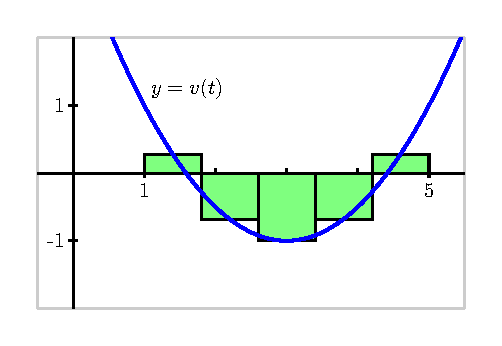
\includegraphics{figures/4_2_Act3Soln.eps}
	\end{center}
	\item Since the net signed area bounded by $v$ on $[1,5]$ represents the total change in position of the object on the interval $[1,5]$, it follows that $M_5$ estimates the total change in position.  Hence, the change in position is approximately $-1.44$ feet.
	\item To estimate the total distance traveled by the object on $[1,5]$, we have to calculate the total area between the curve and the $t$-axis.  Thus,
	$$D \approx \frac{7}{25} \cdot \frac{4}{5} + \frac{17}{25} \cdot \frac{4}{5} + 1 \cdot \frac{4}{5} + \frac{17}{25} \cdot \frac{4}{5} +  \frac{7}{25} \cdot \frac{4}{5} = \frac{292}{125} \approx 2.336.$$
	\item Using appropriate technology, $M_{10} = -1.36$ and $M_{20} = -1.34$.  Further calculations suggest that $M_n \to -\frac{4}{3} = -1.\overline{33}$ as $n \to \infty$, and this number represents the object's total change in position on $[1,5]$.
\ea
\end{activitySolution}
\aftera





 % ACTIVITY
%
%%------------
%% SUMMARY
%%------------
%\begin{summary}
%\item A Riemann sum is simply a sum of products of the form $f(x_i^*) \triangle x$ that estimates the area between a positive function and the horizontal axis over a given interval.  If the function is sometimes negative on the interval, the Riemann sum estimates the difference between the areas that lie above the horizontal axis and those that lie below the axis.
%
%\item The three most common types of Riemann sums are left, right, and middle sums, plus we can also work with a more general, random Riemann sum.  The only difference among these sums is the location of the point at which the function is evaluated to determine the height of the rectangle whose area is being computed in the sum.  For a left Riemann sum, we evaluate the function at the left endpoint of each subinterval, while for right and middle sums, we use right endpoints and midpoints, respectively.
%
%\item The left, right, and middle Riemann sums are denoted $L_n$, $R_n$, and $M_n$, with formulas
%$$L_n = f(x_0) \triangle x + f(x_1) \triangle x + \cdots + f(x_{n-1}) \triangle x = \sum_{i = 0}^{n-1} f(x_i) \triangle x,$$
%$$R_n = f(x_1) \triangle x + f(x_2) \triangle x + \cdots + f(x_{n}) \triangle x = \sum_{i = 1}^{n} f(x_i) \triangle x,$$
%$$M_n = f(\overline{x}_1) \triangle x + f(\overline{x}_2) \triangle x + \cdots + f(\overline{x}_{n}) \triangle x = \sum_{i = 1}^{n} f(\overline{x}_i) \triangle x,$$
%where $x_0 = a$, $x_i = a + i\triangle x$, and $x_n = b$, using $\triangle x = \frac{b-a}{n}$.  For the midpoint sum, $\overline{x}_{i} = (x_{i-1} + x_i)/2$.
%\end{summary}

\cleardoublepage
